% Included from both -slides and -handout versions.

\mode<presentation>
{
  \usetheme{default}
  \useoutertheme{infolines}
}

\usepackage[english]{babel}
\usepackage[latin1]{inputenc}
\usepackage{graphicx}
\usepackage{times}
\usepackage[T1]{fontenc}
\usepackage{fancyvrb}
\usepackage{hyperref}
\usepackage{listings}
\begin{document}
\lstset{language=C, escapeinside={(*@}{@*)}, numbers=left,
  basicstyle=\tiny, showspaces=false, showtabs=false}

\title{L41: Lab 3 - Micro-architectural implications of IPC}
\author{Dr Robert N. M. Watson}
\date{12 November 2015}

\begin{frame}
  \titlepage
\end{frame}

\section{Introduction}

\begin{frame}
  \frametitle{L41: Lab 3 - Micro-architectural implications of IPC}

  \begin{itemize}
    \item Hardware performance counters
    \item Extending Lab 2 from OS effects to architecture/micro-architecture
    \item Gather further data for assessed \textit{Lab Report 2}
  \end{itemize}
\end{frame}

\begin{frame}
  \frametitle{Hardware performance counters}

  \begin{itemize}
    \item Seems simple enough:
    \begin{itemize}
      \item Source code compiles to instructions
      \item Instructions are executed by the processor
    \end{itemize}

    \pause
    \bigskip

    \item But some instructions take longer than others:
    \begin{itemize}
      \item Register-register operations generally single-cycle (or less)
      \item Multiply and divide may depend on the specific numeric values
      \item Floating point may take quite a while
      \item Loads/stores cost different amounts depending on TLB/cache use
    \end{itemize}

    \pause
    \bigskip

    \item Optimisation is therefore not just about reducing instruction count
    \begin{itemize}
      \item Optimisation must take into account micro-architectural effects
      \item TLB/cache effects tricky as they vary with memory footprint
      \item How can we tell when the cache overflows?
    \end{itemize}

    \pause
    \bigskip

    \item Hardware performance counters let us directly ask the processor
      about \textit{architectural} and \textit{micro-architectural} events
    \begin{itemize}
      \item \#instructions, \#memory accesses, \#cache misses, DRAM traffic...
    \end{itemize}
  \end{itemize}
\end{frame}

\begin{frame}
  \frametitle{Sketch of ARM Cortex A8 memory hierarchy}

  \begin{itemize}
    \item \textit{Architectural} refers to an ISA-level view of execution
    \item \textit{Micro-architectural} refers to behaviours below the ISA
  \end{itemize}

  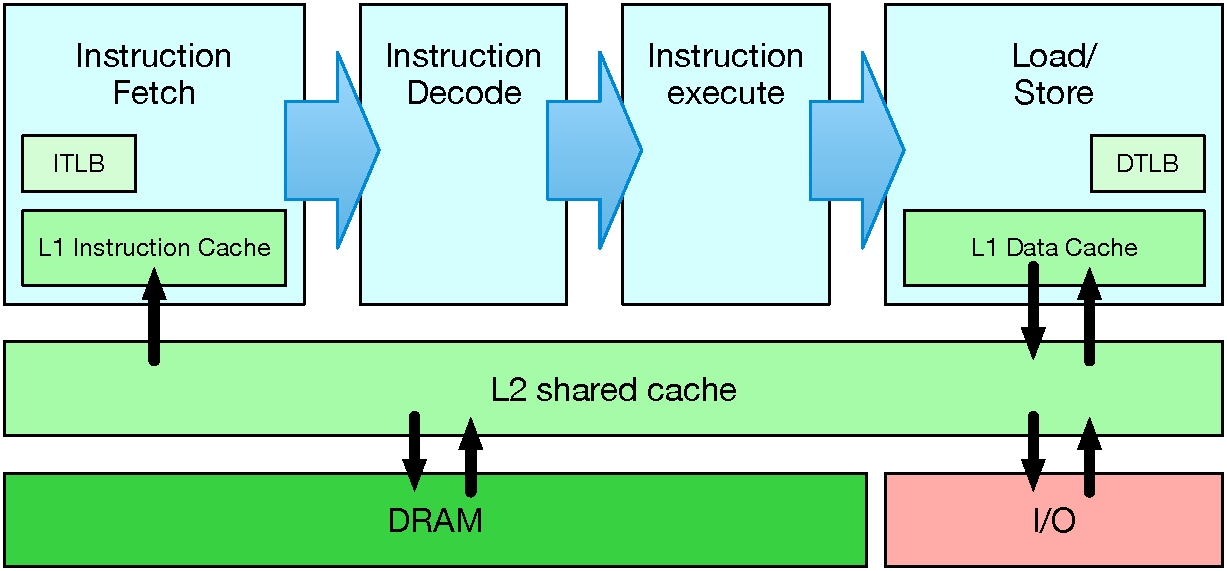
\includegraphics[width=\textwidth]{../../figures/processor-pipeline}

  \begin{scriptsize}
    This is a very, very rough sketch indeed!
  \end{scriptsize}

\end{frame}

\begin{frame}[fragile]
  \frametitle{The benchmark -- now with PMC}

  \begin{scriptsize}
\begin{verbatim}
root@beaglebone:/data/ipc # ./ipc-static 
ipc-static [-Bqsv] [-b buffersize] [-i pipe|socket]
  [-P l1d|l1i|l2|mem|tlb|axi] [-t totalsize] mode

Modes (pick one - default 1thread):
    1thread                IPC within a single thread
    2thread                IPC between two threads in one process
    2proc                  IPC between two threads in two different processes

Optional flags:
    -B                     Run in bare mode: no preparatory activities
    -i pipe|local          Select pipe or socket for IPC (default: pipe)
    -P l1d|l1i|l2|mem|tlb|axi  Enable hardware performance counters
    -q                     Just run the benchmark, don't print stuff out
    -s                     Set send/receive socket-buffer sizes to buffersize
    -v                     Provide a verbose benchmark description
    -b buffersize          Specify a buffer size (default: 131072)
    -t totalsize           Specify total I/O size (default: 16777216)
\end{verbatim}
  \end{scriptsize}

  \begin{itemize}
    \item \texttt{-P} argument requests profiling of load/store instructions,
      L1 D-cache, L1 I-cache, L2 cache, I-TLB, D-TLB, and AXI traffic
  \end{itemize}
\end{frame}

\begin{frame}[fragile]
  \frametitle{Example: Profile memory instructions}

  \begin{scriptsize}
\begin{verbatim}
root@beaglebone:/data/ipc # ./ipc-static -vP mem -b 1048576 -i local
  1thread
Benchmark configuration:
  buffersize: 1048576
  totalsize: 16777216
  blockcount: 16
  mode: 1thread
  ipctype: socket
  time: 0.084140708

  pmctype: mem
  INSTR_EXECUTED: 25463397
  CLOCK_CYCLES: 46233168
  CLOCK_CYCLES/INSTR_EXECUTED: 1.815672
  MEM_READ: 8699699
  MEM_READ/INSTR_EXECUTED: 0.341655
  MEM_READ/CLOCK_CYCLES: 0.188170
  MEM_WRITE: 7815423
  MEM_WRITE/INSTR_EXECUTED: 0.306928
  MEM_WRITE/CLOCK_CYCLES: 0.169044

194721.45 KBytes/sec
\end{verbatim}
  \end{scriptsize}
\end{frame}

\begin{frame}
  \frametitle{Example: Profile memory instructions}

  \begin{itemize}
    \item Benchmark run pushed 16M data through a socket using 1M buffers
      for reads and writes
    \item Reasonable expectation of load and store memory footprints to be
      16M $\times 2 + \epsilon$ reflecting copies to and from kernel buffers

    \pause
    \bigskip

    \item Word size in ARMv7 is 32 bits
    \item Memory reads (8,699,699) $\times$ 4 = $\approx$32M -- sum of buffer
      accesses in user and kernel memory

    \pause
    \bigskip

    \item Could now query L1, L2 caches: how many of those accesses are in
      each cache, and how does it affect performance?
    \item How does L1, L2 cache miss rate relate to cycles/instruction?
    \item How would DTrace profiling show changed behaviour as
      cycles/instruction goes up?
  \end{itemize}
\end{frame}

\begin{frame}
  \frametitle{Exploratory questions}

  \begin{itemize}
    \item How do requested memory access vary across our six benchmark
      configurations?
    \item How does varying the buffer size (and kernel socket-buffer size)
      impact L1, L2 cache effectiveness?
    \item Under what circumstances would increasing buffer size improve
      performance?
    \item Under what cirucmstances would decreasing buffer size improve
      performance?
  \end{itemize}
\end{frame}

\begin{frame}
  \frametitle{Experimental questions for the lab report}

  \begin{itemize}
    \item How does changing the IPC buffer size affect architectural and
      micro-architectural memory behaviour?
    \item Can we reach causal conclusions about the scalability of pipes vs.
      sockets from processor performance counters?
  \end{itemize}
\end{frame}

\begin{frame}
  \frametitle{This lab session}

  Use this session to continue to build experience:
  \begin{itemize}
    \item Ensure that you can use PMC to collect information about the memory
      subsystem: instructions, cache behaviour, AXI behaviour
    \item Continue data collection for Lab Report 2
    \item Identify \textit{inflection points} where performance trends change
      as a result of architectural or micro-architectural thresholds
    \item Do ask us if you have any questions or need help
  \end{itemize}
  Do ask us if you have any questions or need help
\end{frame}

\end{document}
